
\chapter{Comandi base di Git e Github}

Questa è una breve guida dei principali comandi di Git e GitHub che ho creato a scopo personale. Per farlo ho seguito il video al seguente \href{https://www.youtube.com/watch?v=RGOj5yH7evk}{link}.


\subsection{Creare una Repository partendo da GitHub}
Per prima cosa creiamo una nuova repository direttamente dal sito di GitHub.
Possiamo creare un file direttamente dall'editor online di GitHub.
Sempre dal sito stesso possiamo fare delle modifiche (=commit).


\subsection{Copiare la Repository in Locale}
Apriamo Visual Studio Code e mettiamoci nella cartella dove vogliamo mettere la nostra repository.\\
A questo punto possiamo aprire il terminal direttamente da VS Code. Dal terminal (usando cd) ci posizioniamo nella cartella dove vogliamo copiare la repository che avevamo creato sul sito di GitHub.\\

Per farlo, prima di tutto copiamo dal sito di github il link (SSH) alla repository. Sarà una cosa del genere:

\begin{minted}
[
frame=none,
framesep=2mm,
baselinestretch=1.2,
bgcolor=LightGray,
fontsize=\footnotesize,
linenos
]
{bash}
git@github.com:zaffo1/demo-repo.git
\end{minted}

A questo punto sul terminale (sempre dentro VS) possiamo scrivere:

\begin{minted}
[
frame=none,
framesep=2mm,
baselinestretch=1.2,
bgcolor=LightGray,
fontsize=\footnotesize,
linenos
]
{bash}
git clone git@github.com:zaffo1/demo-repo.git
\end{minted}
Abbiamo appena copiato la repository da GitHub in locale!\\


\subsection{Comandi principali in locale}
Mettiamoci ora nella repository appena copiata. Possiamo verificare che è una cartella di git perché contiene una sottocartella (nascosta) chiamata ".git". Questa sottocartella è quella che contiene tutti gli update che facciamo ai nostri file.\\ 
Per vedere anche le cartelle nascoste (tra cui quella .git) uso il comando:
\begin{minted}
[
frame=none,
framesep=2mm,
baselinestretch=1.2,
bgcolor=LightGray,
fontsize=\footnotesize,
linenos
]
{bash}
la
\end{minted}

Non dobbiamo metterci dentro la cartella nascosta chiamata .git, ma rimanere nella cartella che la contiene. E' qui che creeremo i vari file che di cui vorremo tenere traccia.\\

Per vedere lo stato dei vari file uso il comando:

\begin{minted}
[
frame=none,
framesep=2mm,
baselinestretch=1.2,
bgcolor=LightGray,
fontsize=\footnotesize,
linenos
]
{bash}
git status
\end{minted}

Di base git non terrà traccia di tutti i file nella mia cartella, ma devo specificare quali file deve considerare. Per farlo uso il comando \textbf{git add}. In particolare, se voglio includere tutti i file uso il punto dopo il comando:

\begin{minted}
[
frame=none,
framesep=2mm,
baselinestretch=1.2,
bgcolor=LightGray,
fontsize=\footnotesize,
linenos
]
{bash}
git add .
\end{minted}

Con questo comando ho detto di tener traccia di tutti i file nella cartella.

Altrimenti posso specificare quale file aggiungere a quelli di cui tener traccia, ad esempio:

\begin{minted}
[
frame=none,
framesep=2mm,
baselinestretch=1.2,
bgcolor=LightGray,
fontsize=\footnotesize,
linenos
]
{bash}
git add nomefile.txt
\end{minted}

\textbf{Ricorda:} ogni volta che crei un nuovo file devi dire a git di tenerne traccia usando il comando \textbf{git add}.\\


Dopo aver detto a git quali file tracciare, se uso il comand \textbf{git status} avrò un output simile al seguente:



\begin{minted}
[
frame=none,
framesep=2mm,
baselinestretch=1.2,
bgcolor=LightGray,
fontsize=\footnotesize,
linenos
]
{bash}

On branch main
Your branch is up to date with 'origin/main'.

Changes to be committed:
  (use "git restore --staged <file>..." to unstage)
        modified:   README.md
        new file:   index.html
\end{minted}

I file ora sono tracciati e sono pronti per essere "committed".

A questo punto posso usare il comando:

\begin{minted}
[
frame=none,
framesep=2mm,
baselinestretch=1.2,
bgcolor=LightGray,
fontsize=\footnotesize,
linenos
]
{bash}

git commit -m "messaggio"
\end{minted}

Dove il messaggio dovrebbe contenere informazioni sui cambiamenti che abbiamo effettuato ai nostri file.\\
Se ho bisogno di aggiungere un ulteriore sottomessaggio posso scrivere invece:

\begin{minted}
[
frame=none,
framesep=2mm,
baselinestretch=1.2,
bgcolor=LightGray,
fontsize=\footnotesize,
linenos
]
{bash}

git commit -m "messaggio" -m "ulteriore descrizione"
\end{minted}

A questo punto abbiamo salvato il "commit" in locale, ma ancora non lo abbiamo caricato su GitHub. Per farlo usiamo:

\begin{minted}
[
frame=none,
framesep=2mm,
baselinestretch=1.2,
bgcolor=LightGray,
fontsize=\footnotesize,
linenos
]
{bash}

git push origin main
\end{minted}


\subsection{Creare una Repository in locale}
Finora abbiamo lavorato a partire da una repository creata inizialmente su GitHub. Ora vediamo come fare se vogliamo lavorare partendo direttamente in locale.\\


Creiamo una nuova cartella nella quale vogliamo mettere i nostri file. Per ora è una normalissima cartella, non è una repository di git. Se vogliamo che diventi una cartella di git, da terminale, dopo esserci messi in questa cartella, usiamo il comando:
\begin{minted}
[
frame=none,
framesep=2mm,
baselinestretch=1.2,
bgcolor=LightGray,
fontsize=\footnotesize,
linenos
]
{bash}

git init
\end{minted}

A questo punto possiamo usare tutti i comandi che abbiamo gia visto:
\begin{minted}
[
frame=none,
framesep=2mm,
baselinestretch=1.2,
bgcolor=LightGray,
fontsize=\footnotesize,
linenos
]
{bash}

git add     #per aggiungere file da tracciare
git status  #per vedere lo stato dei file nella cartella
git commit -m "commento" -m "ulteriore commento"    #per effettuare un "commit"
\end{minted}

A questo punto vogliamo caricare il tutto su github, come fare?
Se usiamo il comando 
\begin{minted}
[
frame=none,
framesep=2mm,
baselinestretch=1.2,
bgcolor=LightGray,
fontsize=\footnotesize,
linenos
]
{bash}

git push origin master
\end{minted}

otterrò un errore. GitHub non ha idea di dove caricare questa nostra repository locale.
La cosa più semplice da fare è quindi creare una repository vuota dal sito di GitHub. Una volta creata uscirà una schermata del genere:



\begin{figure}[h]
    \centering
    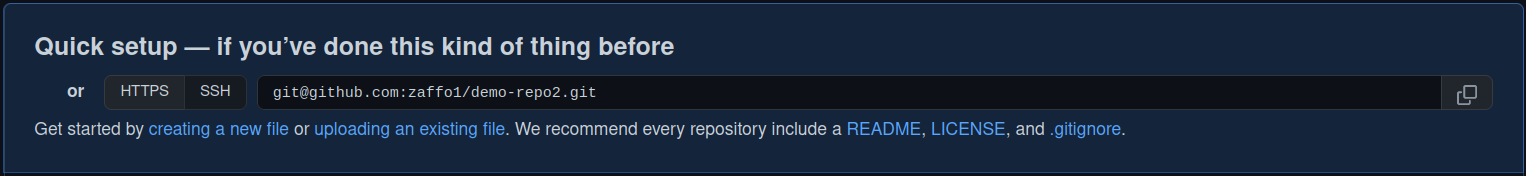
\includegraphics[width=1\textwidth]{images/screenshot_github_tutorial_repo.png}
\end{figure}
\FloatBarrier

Copiamo il link visualizzato e usiamo il comando:

\begin{minted}
[
frame=none,
framesep=2mm,
baselinestretch=1.2,
bgcolor=LightGray,
fontsize=\footnotesize,
linenos
]
{bash}

git remote add origin git@github.com:zaffo1/demo-repo2.git
\end{minted}
 per effettuare il collegamento alla repository su GitHub.
 Possiamo controllare che il collegamento sia avvenuto scrivendo:
 
 \begin{minted}
[
frame=none,
framesep=2mm,
baselinestretch=1.2,
bgcolor=LightGray,
fontsize=\footnotesize,
linenos
]
{bash}

git remote -v
\end{minted}

dovremmo ottenere una cosa del genere:
\begin{minted}
[
frame=none,
framesep=2mm,
baselinestretch=1.2,
bgcolor=LightGray,
fontsize=\footnotesize,
linenos
]
{bash}

origin  git@github.com:zaffo1/demo-repo2.git (fetch)
origin  git@github.com:zaffo1/demo-repo2.git (push)
\end{minted}

Adesso posso usare il comando:

\begin{minted}
[
frame=none,
framesep=2mm,
baselinestretch=1.2,
bgcolor=LightGray,
fontsize=\footnotesize,
linenos
]
{bash}

git push -u origin master
\end{minted}
il pezzo "-u" serve per poter impostare di default questa destinazione. Cosicché le prossime volte mi basterà scrivere
\begin{minted}
[
frame=none,
framesep=2mm,
baselinestretch=1.2,
bgcolor=LightGray,
fontsize=\footnotesize,
linenos
]
{bash}
git push 
\end{minted}

Abbiamo caricato la nostra repository su GitHub!

\textbf{Nota}: a volte ho usato \textbf{main} e a volte \textbf{master}. Bisogna essere consistenti.
\subsection{Git Workflow}

\begin{figure}[h]
    \centering
    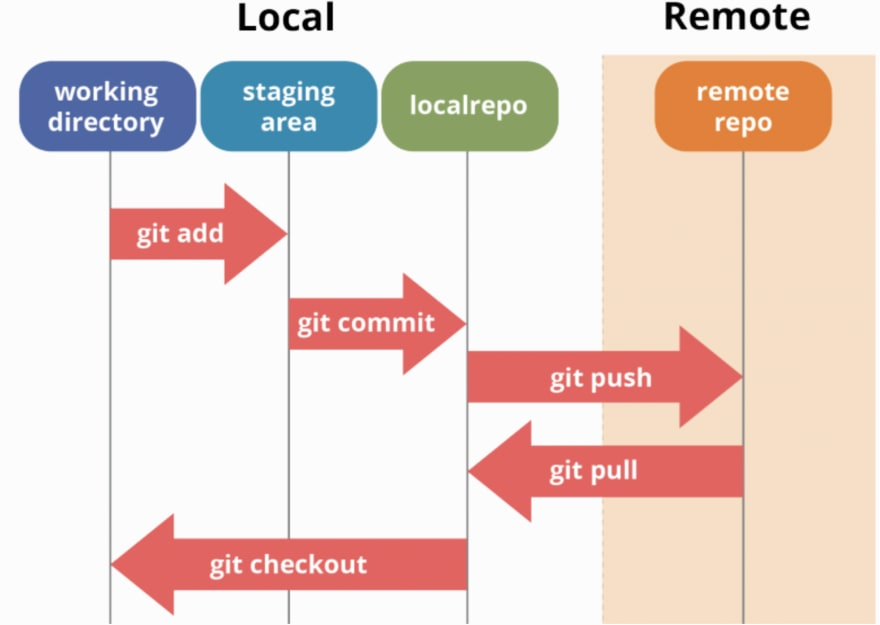
\includegraphics[width=0.6\textwidth]{images/git_workflow.jpeg}
\end{figure}
\FloatBarrier

%\subsection{Git Branching}

%31:00

%guarda anche: https://www.youtube.com/watch?v=8JJ101D3knE
